\documentclass[12pt]{article}
\usepackage{graphicx}
\usepackage{xurl}
\usepackage{xcolor}
\usepackage{listings}
\usepackage{verbatim}

\newenvironment{metaverbatim}{\verbatim}{\endverbatim}
\DeclareUnicodeCharacter{001B}{\textendash}

\definecolor{mygray}{rgb}{0.4,0.4,0.4}
\definecolor{mygreen}{rgb}{0,0.8,0.6}
\definecolor{myorange}{rgb}{1.0,0.4,0}

\lstset{
basicstyle=\footnotesize\sffamily\color{black},
commentstyle=\color{mygray},
frame=single,
numbers=left,
numbersep=9pt,
numberstyle=\color{mygray},
keywordstyle=\color{mygreen},
showspaces=false,
showstringspaces=false,
stringstyle=\color{myorange},
tabsize=2
}

\begin{document}

\thispagestyle{empty}
\begin{center}
    
\includegraphics[width=0.3\linewidth]{./images/Reading_shield.png}
    \par
    \large{University of Reading}\par
    \vspace{0.5 cm}
    {Department of Computer Science}\par
%Title
    \vspace{0.5 cm}
    {\Large     CS1PC20 - Programming in C++   \par} % Course ID and Project Title
    {           Coursework 4 - Modifying a Game in C/C++    \par} % Coursework Subtitle
%Author's name
    {\Large     Ruben j. Lopes   \par} % First Name And Surname
%Degree
    \begin{center}
        \begin{tabular}{p{0.35\linewidth}p{0.8\linewidth}}
            Module Code: &         CS1PC20           \\ 
            Report Title: &        Coursework 4           \\  
            Student Number: &      30021591           \\
            Date: &                28th March 2022           \\
            hrs spent: &           25hr           \\
            Git Repository: &      \url{https://csgitlab.reading.ac.uk/il021591/cs1pc20_Spring_Project.git}         \\ 
            Lecturer: &            Dr Ashraf Mahmud           \\
            Weighting of the Assignment: & 30\% \\
            Assignment evaluation: & Impoved understanding and confidance programming in C. Learned the impartance of commenting and documentation for mantainance. 
        \end{tabular}
    \end{center}
\end{center}

\tableofcontents
\section*{Declaration}
I, Ruben Lopes, of the Department of Computer Science, University of Reading,
corm that all the sentences, gures, tables, equations, code snippets, artworks, and illus-
trations in this report are original and have not been taken from any other person's work,
except where the works of others have been explicitly acknowledged, quoted, and referenced.
I understand that if failing to do so will be considered a case of plagiarism. Plagiarism is a
form of academic misconduct and will be penalised accordingly.

\hspace*{0pt}\hfill --- Ruben Lopes 
\break{}
\hspace*{0pt}\hfill February 1, 2021

\newpage

\section{Introduction}
The goal of this project was to demonstrate our capacity to analyse, create, and implement current C/C++ code to add new features. The SLD2 library was included in the skeleton code for the basic game which we had to utilize to run the graphical components of the game. The Theme I used throughout was a moon-based space game. Making the player in this case a human astronaut. The main objective for the player in this game is to collect all the neon blue orbs on each map. The player will have to navigate across the maps using platforms and blocks and will have to avoid taking damage from the aliens.

I have implemented about five features, four new maps and have created twenty-two textures. The features that I have implemented were the ability for the player to choose to do a different map or level. Additionally, a menu screen is displayed at the start of the game to allow the user to choose one of the five maps/levels made available to them. Moving Aliens that decrees the players health or kills the player when the character interacts with it was also implemented and the player was given the ability to shoot when the ‘shift’ button was held, this allowed the player to kill the Alien. In addition to functional change, I have also changed the texture of the blocks, character, background, and platform to fit the theme of the game.

The Programming style used by me is mainly imperative as C was predominately used to implement all the new features. Although for components such as entities structs were used to store objects such as enemies and player information so it can be more accessible to other functions. The public functions in the skeleton code and some of the ones I implemented were stored in the commons.h file. 

In this report, I will go through the development decisions and design choices I made for these features I implemented. This report will consist of four additional components. In design I will be focusing on the UI and textures and the objects and its features. In the implementation and development section I will go into more detail about each feature and describe the development process of each feature more clearly, additionally, I will Justify my changes compared to keeping the original design. And finally, describe improvements or alternative features I could have used in the conclusions. The difference of code will also be available at the end of this document, comparing the original skeleton code provided to the code that I wrote.

\newpage

\section{Design}
The new maps or levels encourage gamers to explore the game in a variety of terrains. The addition of aliens made the game more difficult, and this feature also permitted the addition of laser weapons. The alien's movement is implemented using the same mechanism as the platforms provided in the skeleton code. With a few changes, the shooting functionality was also easily implemented utilizing the pre-existing struct. Because having infinite weapon ammo would make the game easy, I set a restriction to how much it can be used by utilizing a counter and only allowing one hundred bullets when the player spawns, however, the player earns more bullets when orbs are gathered.

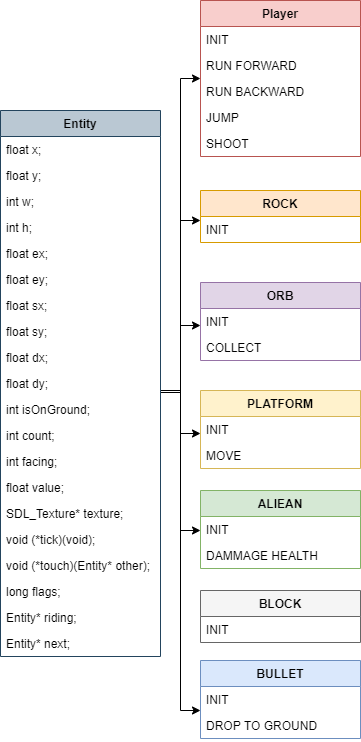
\includegraphics[width=.35\linewidth]{images/UML.png}
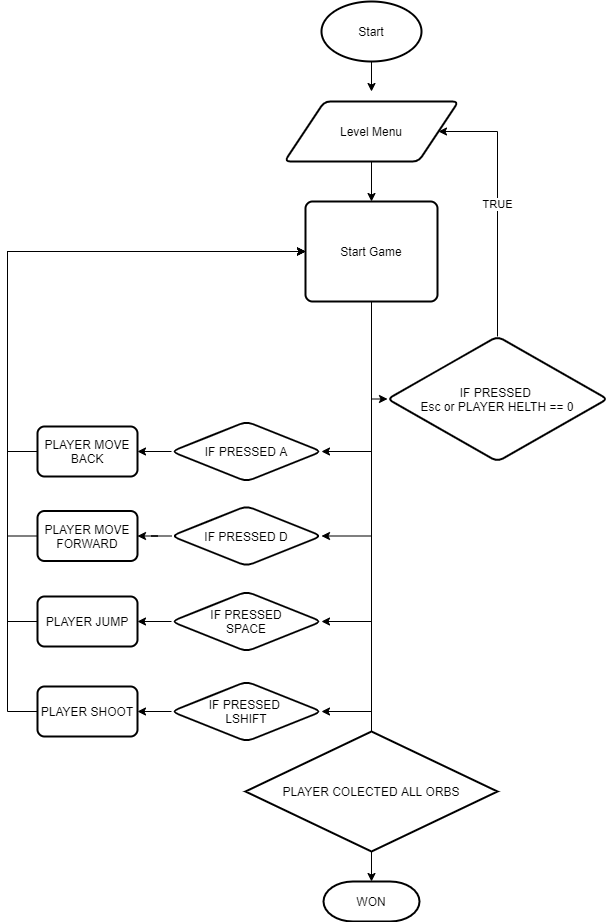
\includegraphics[width=.45\linewidth]{images/top-level.png}

The controls to the player are listened for in the game loop once the game starts. To interact with the game, the user can then move, shoot, or jump using W A S D Right Shift or spacebar. If the player gathers all of the orbs on the map, the game finishes, and the level is completed. If the player touches the alien, it loses health, and if it falls below zero, the game terminates, and the player is returned to the menu. This is visualized using the flowchart below.

\newpage

\section{Implementation and development}
Since the core of the programming was provided to us in the skeleton code to add new features, I used the pre-existing code and designed and built the additional features based on it. Firstly, I developed separate files called attack.c, emeny.c, and menu.c for the three primary new features. I made some other adjustments after adding it to the commons header file and the struct file. 

\subsection{New Maps or Levels}
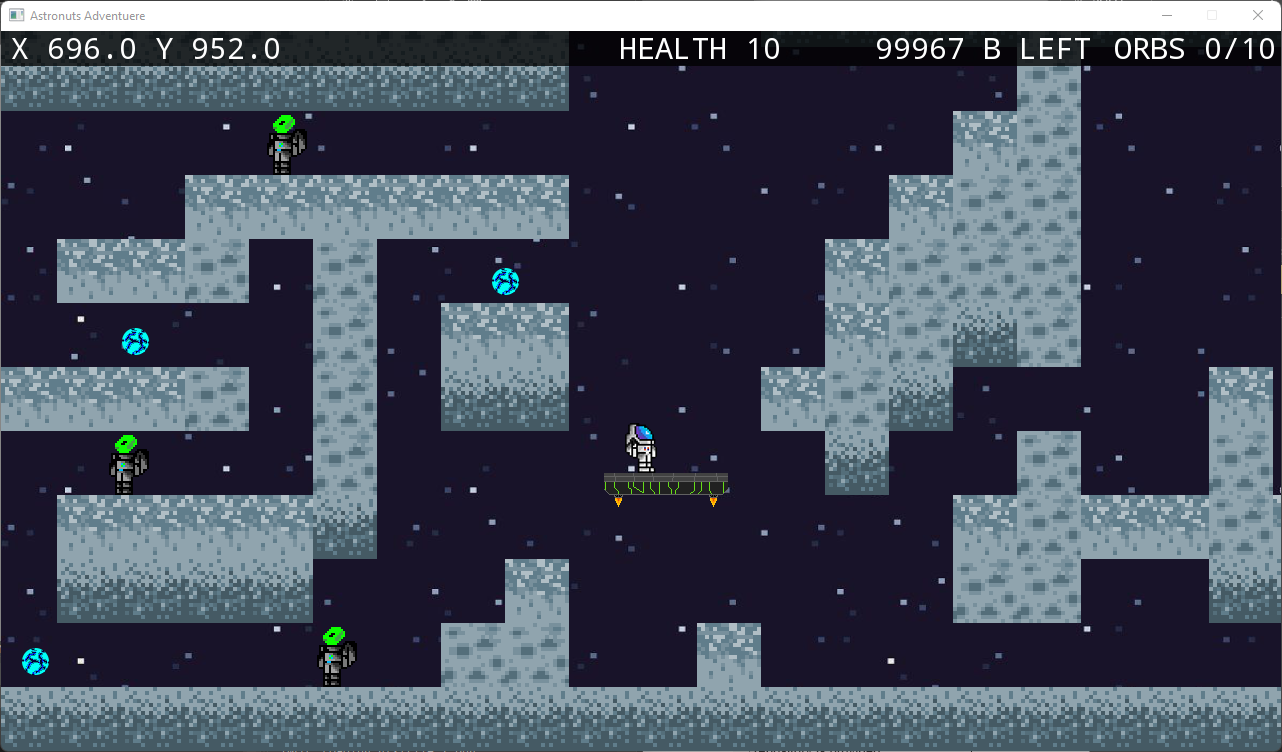
\includegraphics[width=1\linewidth]{images/ss.png}
We were provided a single map in the skeleton code. These were set up using a 40 by 60 number matrix ranging from 1 to 7. The initmap function then read this by calling the io.c file. The map was created, and the entities from the entX.dat folder were placed depending on their coordinates.
These files served as the foundation for the additional four maps I produced. Similarly, to the maps, I had to create four more entity files to add the entities to the new maps. The Alien entity was also updated to be able to be added using this method. during the map making process I found it difficult to determine the correct coordinates while creating the map, so I used the drawText method to print out the players' x and y coordinates. This, however, was solely for development and testing and will be deleted in the final version.


\subsection{Game Textures and theme}

\begin{tabular}{ll}
    Astronaut Right Still & 
\includegraphics[width=.08\linewidth]{C:/Users/ru4en/OneDrive/Desktop/SpringProjectx/gfx/astroF1.png} \\
    Astronaut Left Still & 
\includegraphics[width=.08\linewidth]{C:/Users/ru4en/OneDrive/Desktop/SpringProjectx/gfx/astroB1.png} \\
    Astronaut Right Walk & 
\includegraphics[width=.08\linewidth]{C:/Users/ru4en/OneDrive/Desktop/SpringProjectx/gfx/astroF2.png} \\
    Astronaut Left Walk & 
\includegraphics[width=.08\linewidth]{C:/Users/ru4en/OneDrive/Desktop/SpringProjectx/gfx/astroB2.png} \\
    Astronaut Right Jump & 
\includegraphics[width=.08\linewidth]{C:/Users/ru4en/OneDrive/Desktop/SpringProjectx/gfx/astroFJ.png} \\
    Astronaut Left Jump & 
\includegraphics[width=.08\linewidth]{C:/Users/ru4en/OneDrive/Desktop/SpringProjectx/gfx/astroBJ.png} \\
\end{tabular}
\begin{tabular}{ll}
    Alien Right Still & 
\includegraphics[width=.08\linewidth]{C:/Users/ru4en/OneDrive/Desktop/SpringProjectx/gfx/alienB1.png} \\
    Alien Left Still & 
\includegraphics[width=.08\linewidth]{C:/Users/ru4en/OneDrive/Desktop/SpringProjectx/gfx/alienF1.png} \\
    Rock 1 & 
\includegraphics[width=.08\linewidth]{C:/Users/ru4en/OneDrive/Desktop/SpringProjectx/gfx/rock1.png} \\   
    Rock 2 & 
\includegraphics[width=.08\linewidth]{C:/Users/ru4en/OneDrive/Desktop/SpringProjectx/gfx/rock2.png} \\
    Lazar Shot & 
\includegraphics[width=.08\linewidth]{C:/Users/ru4en/OneDrive/Desktop/SpringProjectx/gfx/shot.png} \\
    Orb & 
\includegraphics[width=.08\linewidth]{C:/Users/ru4en/OneDrive/Desktop/SpringProjectx/gfx/spr.png} \\
    Moon Topsoil & 
\includegraphics[width=.08\linewidth]{C:/Users/ru4en/OneDrive/Desktop/SpringProjectx/gfx/tile_1.png} \\
    Moon Rock & 
\includegraphics[width=.08\linewidth]{C:/Users/ru4en/OneDrive/Desktop/SpringProjectx/gfx/tile_2.png} \\
    Moon Bedrock & 
\includegraphics[width=.08\linewidth]{C:/Users/ru4en/OneDrive/Desktop/SpringProjectx/gfx/tile_3.png}
\end{tabular}

The controls to the player are listened for in the game loop once the game starts. To interact with the game, the user can then move, shoot, or jump using W A S D Right Shift or spacebar. If the player gathers all of the orbs on the map, the game finishes, and the level is completed. If the player touches the alien, it loses health, and if it falls below zero, the game terminates, and the player is returned to the menu. This is visualized using the flowchart below.



The game, as indicated in the introduction, is based on a shooting game with a moon theme. I choose pixel art as the art style for this game. All of the textures in the game were created in Photoshop using a certain colour palette and aspect ratio. The player includes six distinct texture pictures for the left and right positions of the three functions it may perform: stand, walk, and leap. Similarly, the alien had textures on both the left and right sides. The platform was designed to seem like an industrial Si-Fi spaceship platform. Three tiles were made with topsoil, dirt, and bedrock designs to make the terrain look like the moon. Rocks were added for astatic, and the pizza was also changed to a blue orb to fit the theme.

\subsection{Game Menu}
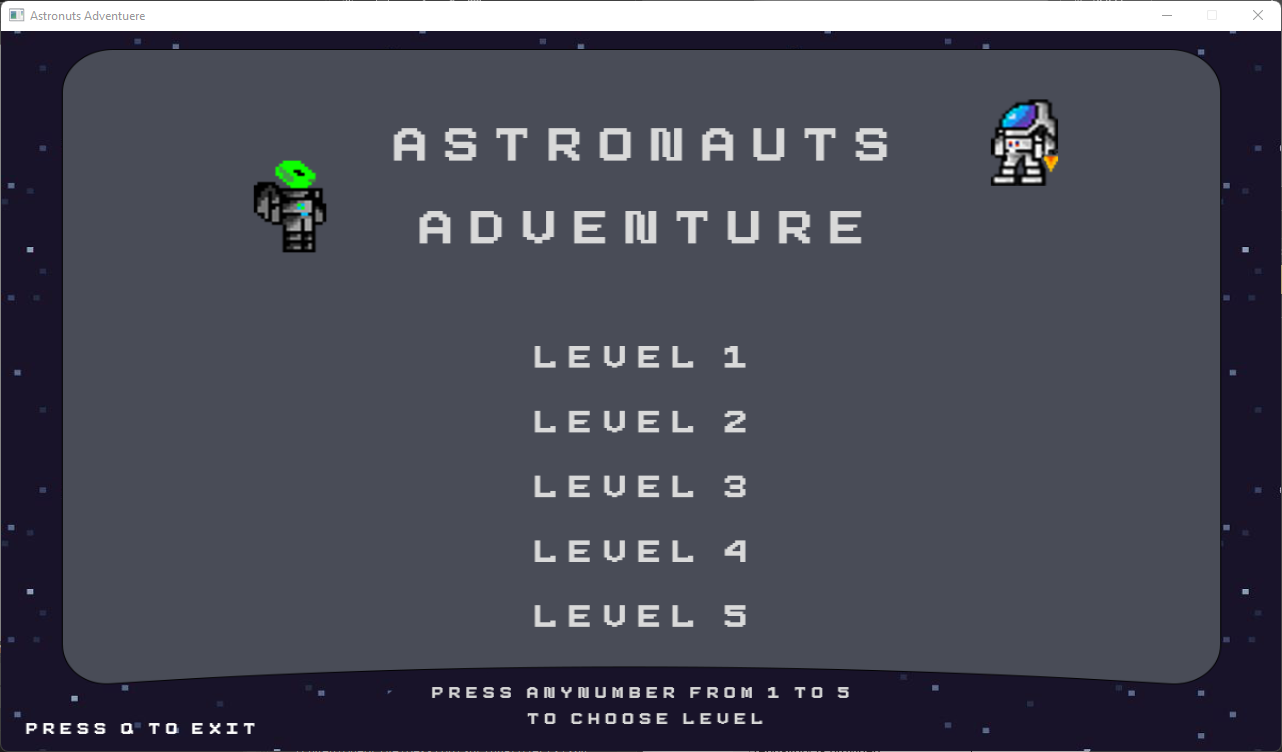
\includegraphics[width=1\linewidth]{images/ss5.png}
The game menu is comprised of a basic backdrop image created in Photoshop. In the same way as the game does, this loops until any number from 1 to 5 is pressed to begin the level. Alternatively, Q could be pressed to exit the application. Players may also return to this menu by pressing esc during the game, although their progress will be lost. 

\lstinputlisting[language=c]{C:/Users/ru4en/OneDrive/Desktop/SpringProjectx/src/menu.c}

 \newpage

 \subsection{Player Attacks (Shooting)}
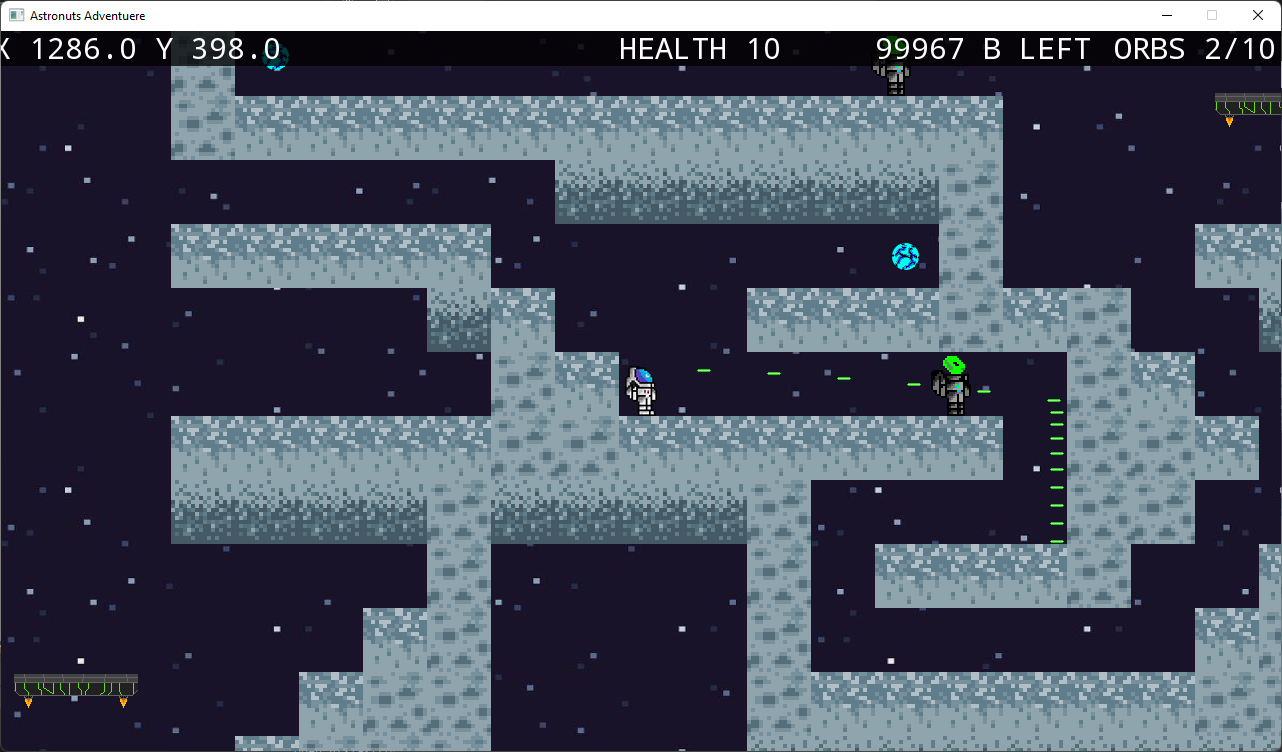
\includegraphics[width=1\linewidth]{images/ss1.png}
The shooting functionality utilises the entity struct to create bullets. When a collision is detected, these bullets activate the touch function. If it collides with an entity, it will cause harm, and if it collides with the ground, it will disappear. The bullet's velocity is stored in the struct's dy variable, which uses the physics of all the other entities previously supplied and is inverted according on the player's location, for example, if the player fires towards the left, the bullet is shot from the left. The bullets are also restricted to one hundred every game and will – 1 for each shot until they reach 0, and the player will be unable to fire the laser gun unless an orb is obtained, which grants the player +5 bullets.
\lstinputlisting[language=c]{C:/Users/ru4en/OneDrive/Desktop/SpringProjectx/src/attack.c}
 
 \newpage

\subsection{Enemy (Aliens)}
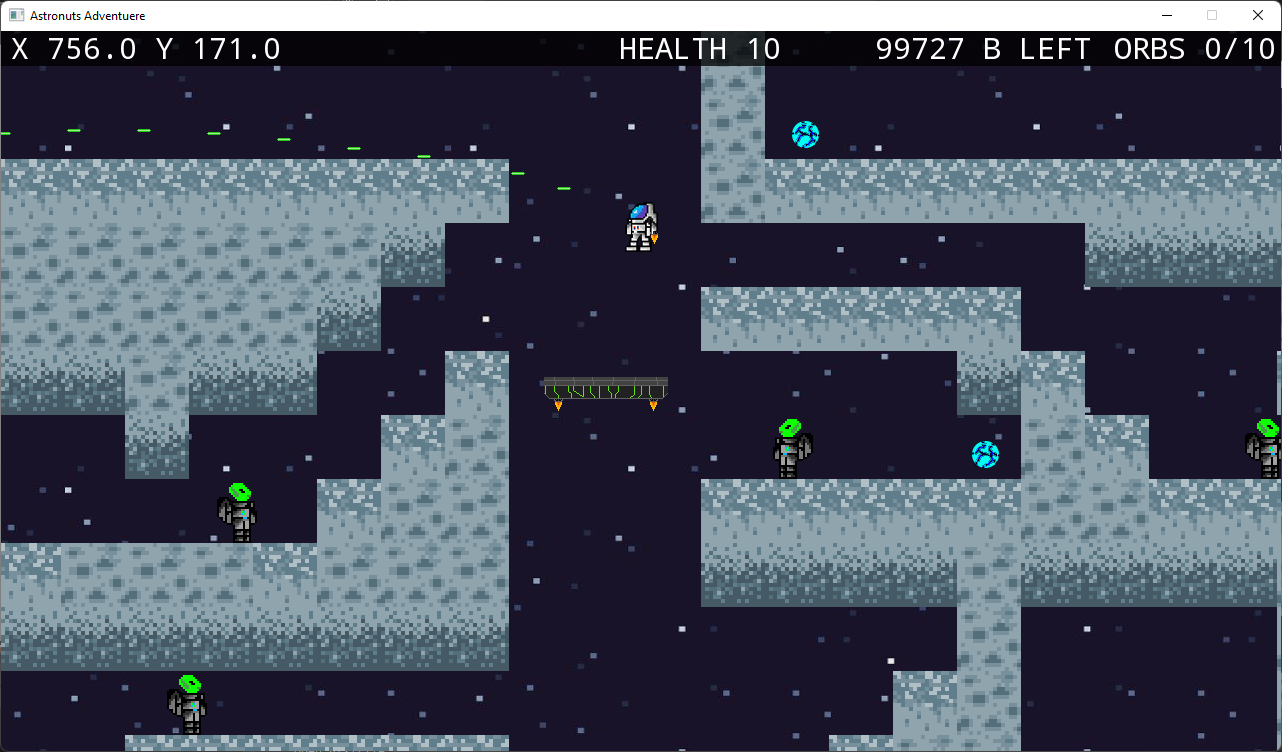
\includegraphics[width=1\linewidth]{images/ss3.png}
The aliens were designed to add a level of difficulty to the game. Alien movement from sx to ex is similar to platforms and may be set in the etntery.dat file. If the player fires at these aliens, they will receive damage, and if the player touches them, they will kill the player instantaneously. The aliens have two textures, which are kept in an array of SDL texture. It likewise made use of the same struct as the other entities. 
\lstinputlisting[language=c]{C:/Users/ru4en/OneDrive/Desktop/SpringProjectx/src/enemy.c}
  
\newpage

\section{Conclusions}

In conclusion this coursework project helped me understand the importance of reliability of code and the steps to maintain and update repositories. I Also helped me to improve my understanding as well as confidence C and improved my problem-solving skill. Besides programming, designing textures was also something I learned. If I were to do this project again, I would plan out a game more thoroughly and use a software development life cycle such as sprint and a Kanban board to manage the project. Furthermore, I could have more comments and audited the progress better to reduce setbacks in managing a project of a multiple files. 
\par
I have recognized that I could improve my productivity if I learn to use Git and a testing framework as I struggled to maintain my code and often failed to remember where I last modified code. And this could also aid in have a more inadept testing of features as I could test and push iteratively.

\newpage

\section{Git repository diff}
\lstinputlisting[language=c]{C:/Users/ru4en/OneDrive/Desktop/SpringProjectx/src/proj.diff}
\newpage

\section*{Sources and References}
\input{chapters/Sources_and_references}

\end{document}